\chapter{Path Tracing}\label{chp:path-tracing}
From this chapter, we are going to discuss some approaches of global illumination. The goal of this article is try to discuss all the knowledge about GI a game developer should know. So we can choose the appropriate algorithm for our game or game engine.  

We introduce these algorithms by the order of rendering quality, which also means performance because high quality image costs more rendering time. We first detail the four main techniques from which most other techniques derive are path tracing, radiosity, photon mapping and instant radiosity. These techniques are generally considered to be able to generate high quality global illumination in practice. But we should note that only path tracing can generate unbiased result. Although these algorithms are expensive, we also show some applications of them can reach interactive even real-time needs. 



\section{Ray Tracing and the History} 
In nature, a light source emits a ray of light which travels, eventually, to a surface that interrupts its progress. A surface may absorb part of the light ray, resulting in a loss of intensity of the reflected and/or refracted light. It might also reflected all of the light ray, in one or more directions. If the surface has any transparent or translucent properties, it refracts portion of the light beam into itself in a different direction while absorbing some (or all) of the spectrum.

\begin{figure}\label{f:path-tracing}
	\sidecaption
	\includegraphics[width=.65\textwidth]{graphics/gi/path-1}
	\caption{The ray tracing algorithm builds an image by extending rays into a scene.}
\end{figure}

\textit{Ray tracing} is the construction of a synthesized image by constructing light transport paths between the camera, through the screen pixels, to the light source in the scene. See figure \ref{f:path-tracing}.

Simple \textit{ray casting} \cite[-7mm]{a:Sometechniquesforshadingmachinerenderingsofsolids} with \textit{shadow rays} to point light source implements the following approximation of the rendering equation:

\begin{equation}
	L(p,\omega_o)=L_e(p, \omega_o)+\sum_{i=1}^{N_L}L(p,\omega_i) f_r(p,\omega_o,\omega_i)|cos\theta_i|
\end{equation}

Previous algorithms traced rays from the eye into the scene until they hit an object, but determined the ray color without recursively tracing more rays. Whitted \cite{a:ray-tracing} continued the process. When a ray hits a surface, it can generate up to three new types of rays: reflection, refraction, and shadow, see figure \ref{f:recursive-ray-tracing}. 

\begin{figure}\label{f:recursive-ray-tracing}
	\sidecaption	
	\includegraphics[width=0.6\textwidth]{graphics/gi/path-2}
	\caption{A single ray traces from the eye through the screen into a scene. It generates four rays; two to the two lights and one reflection and one refraction ray. These rays continue on, possibly spawning yet more rays (Image courtesy of "Real-Time Rendering(3rd edition)").}
\end{figure}

This determinsitic form of ray tracing is referred to as \textit{Whitted-style ray tracing} or \textit{recursive ray tracing}, which implements the following approximation of the rendering equation:

\begin{equation}
\begin{aligned}
	L(p,\omega_o)=&L_e(p, \omega_o)+\sum_{i=1}^{N_L}L(p,\omega_i) f_r(p,\omega_o,\omega_i)|cos\theta_i|\\
	&+L_r(p,\omega_r)f_r(p,\omega_o,\omega_r)|cos\theta_r|
\end{aligned}
\end{equation}

Whitted-style ray tracing adds indirect lighting to the direct lighting, but this is limited to pure specular transmissive and reflective surfaces. Because it samples the value of the integrand at a single point in the domain. The BRDF in the recursive part of the above formulation is thus a Dirac function.

This limitation is alleviated in \textit{distribution ray tracing}, introduced by Cook \cite[-6mm]{a:DistributedRayTracing} in 1984. This algorithm approximates glossy reflections using an integral over the surfaces in the scene, and soft shadows using an integral over the surface of each light source. Because the integrations are approximated by Monte Carlo method, it is also called \textit{stochastic ray tracing}, which implements the following approximation of the rendering equation:

\begin{equation}
\begin{aligned}
	L(p,\omega_o)=&L_e(p, \omega_o)+\sum_{i=1}^{N_L}\int_{\Omega_i}L(p,\omega_i) f_r(p,\omega_o,\omega_i)|cos\theta_i|d\omega_i\\
	&+\int_{\Omega_r}L_r(p,\omega_r)f_r(p,\omega_o,\omega_r)|cos\theta_r|d\omega_r
\end{aligned}
\end{equation}

In distribution ray tracing, illumination rays are distributed according to the illumination function $L$ (area of the light source $L$); Reflected rays are distributed according to the reflectance function. see figure \ref{f:distribution-ray-tracing}. 

\begin{figure}\label{f:distribution-ray-tracing}
\sidecaption
	\includegraphics[width=0.65\textwidth]{graphics/gi/path-3}
	\caption{Typical distribution ray path.}
\end{figure}

In figure \ref{f:distribution-ray-tracing}, to calculate every single ray (shadow, reflected or refracted ray), some directions are sampled, which forms a tree of rays and cost lots of time. So it's impossible to include indirect diffuse lighting which needs to integral over the whole hemisphere for every single ray.

Kajiya generalizes the concept of stochastic sampling, by randomly sampling all possible light transport paths \cite[5mm]{a:TheRenderingEquation}. His \textit{path tracing} algorithm is able to render most natural phenomena, including diffuse reflections, diffraction, indirect light and caustics.




\section{The Surface Form of The Rendering Equation}\label{sec:surface-form}
Although inspired by distributed ray tracing, path tracing using a different strategy to sample points in the scene. To know it, we'd better discuss the surface form of the rendering equation first, which is the key to understand path tracing and the reason why path tracing can improve the performance for indirect diffuse lighting. This way to learn and understand path tracing mainly comes from the book "Physically Based Rendering, Second Edition" \cite{b:pbrt}.

The most commonly used formulation of the rendering equation is the \textit{hemispherical formulation}, which integral the radiance over the directions of the hemisphere:

\begin{equation}\label{e:hemisphere-formulation}
	L(p,\omega_o)=L_e(p,\omega_o)+\int_{\Omega}f(p,\omega_o,\omega_i)L(t(p,\omega_i),-\omega_i)|cos\theta_i|d\omega_i
\end{equation}

where $t(p,\omega)$ is called \textit{ray-casting function} that computes the first surface point $p^{'}$ intersected by a ray from $p$ in the direction $\omega$.

One reason why the LTE as written in equation \ref{e:hemisphere-formulation} is complex is that \textbf{the relationship between geometric objects in the scene is implicit in the ray-tracing operator $t(p,\omega)$}. Making the behavior of the ray-tracing operator explicit in the integrand will shed some light on the structure of this equation. \textbf{To do this, we will rewrite equation \ref{e:hemisphere-formulation} as an integral over \textit{area} instead of an integral over directions on the sphere}.

\begin{figure}\label{f:three-point-form}
	\sidecaption
	\includegraphics[width=0.6\textwidth]{graphics/gi/path-4}
	\caption{The three-point form of the light transport equation converts the integral to be over the domain of points on surfaces in the scene, rather than over directions over the sphere. It is a key transformation for deriving the path integral form of the light transport equation (Image courtesy of "Physically-based Rendering, Second Edition").}
\end{figure}

First, we define exitant radiance from a point $p^{'}$ to a point $p$ by

\begin{equation*}
	L(p^{'}\to p)=L(p^{'},\omega)
\end{equation*}

if $p^{'}$ and $p$ are mutually visible and $\omega=\widehat{p-p^{'}}$. We can also write the BRDF at $p^{'}$ as 

\begin{equation*}
	f(p^{''}\to p^{'}\to p)=f(p^{'},\omega_o,\omega_i)
\end{equation*}

where $\omega_i=\widehat{p^{''}-p^{'}}$ and $\omega_o=\widehat{p^{'}-p}$, see figure \ref{f:three-point-form}.

We also need to transform solid angle to area, that is $|cos\theta^{'}|/r^2$. Combing this change-of-variables term, the original $|cos\theta|$ term from the LTE, and also a binary visibility function $V$ ($V=1$ if the two points are mutually visible, and $V=0$ otherwise) into a single geometric coupling term $G(p\leftrightarrow p^{'})$:

\begin{equation*}
	G(p\leftrightarrow p^{'})=V(p\leftrightarrow p^{'})\frac{|cos\theta||cos\theta^{'}|}{||p-p^{'}||^2}
\end{equation*} 

Substituting these into the light transport equation and converting to an integral, we have

\begin{equation}\label{e:integral-over-area}
	L(p^{'}\to p)=L_e(p^{'}\to p)+\int_A f(p^{''}\to p^{'}\to p)L(p^{''}\to p^{'})G(p\leftrightarrow p^{'})dA(p^{''})
\end{equation}

where $A$ is all of the surfaces of the scene.

Although equation \ref{e:hemisphere-formulation} and \ref{e:integral-over-area} are equivalent, they represent two different ways of approaching light transport. and which is also the different between ray tracing and path tracing. To evaluate equation \ref{e:hemisphere-formulation} with Monte Carlo, we would sample a number of directions from a distribution (BRDF or light source area) of directions on the sphere and cast rays to evaluate the integrand. For equation \ref{e:integral-over-area}, however, we would choose a number of points on surfaces according to a distribution over surface area and compute the coupling between those points to evaluate the integrand, tracing rays to evaluate the visibility term $(p\leftrightarrow p^{'})$. We will discuss how to sample these points later, but before that we need to know what is a path.



\subsection{Integral Over Paths}
We now change the area formulation to a path form, a sum over light-carrying paths of different lengths, by repeatedly substituting the right-hand side of the equation into the $L(p^{''}\to p^{'})$ term inside the integral. The equation becomes

\begin{equation*}
	\begin{aligned}
		L(p_1\to p_0)=&L_e(p_1\to p_0)\\
		&+\int_AL_e(p_2\to p_1)f(p_2\to p_1\to p_0)G(p_2\leftrightarrow p_1)dA(p_2)\\
		&+\int_A\int_A L_e(p_3\to p_2)f(p_3\to p_2\to p_1)G(p_3\leftrightarrow p_2)\\
		&\qquad\qquad \times f(p_2\to p_1\to p_0)G(p_2\leftrightarrow p_1)dA(p_3)dA(p_2)+...
	\end{aligned}
\end{equation*}

where $p_1$ is the first point on a surface along the ray from $p_0$ in $p_1-p_0$, and $p_0$ is the eye point.

Each term on the right of this equation represents a \textit{path} of increasing length. For example, the third term is illustrated in figure \ref{f:three-point-form-1}. The integral over all such $p_2$ and $p_3$ gives the total contribution of paths of length four to radiance arriving at camera.

\begin{figure}\label{f:three-point-form-1}
	\includegraphics[width=0.9\textwidth]{graphics/gi/path-5}
	\caption{The integral over all points $p_2$ and $p_3$ on surfaces in the scene given by the light transport equation gives the total contribution of two bounce paths to radiance leaving $p_1$ in the direction of $p_0$. The components of the product in the integrand are shown here: the emitted radiance from the light, $L_e$; the geometric terms between vertices, $G$; and scattering from the BRDFs, $f$ . (Image courtesy of "Physically-based Rendering, Second Edition").}
\end{figure}

This infinite sum can be written compactly as 

\begin{equation}\label{e:path-form}
	L(p_1\to p_0)=\sum_{n=1}^{\infty}P(\bar{p}_n)
\end{equation}

where $P(\bar{p}_n)$ gives the amount of radiance scattered over a path $\bar{p}_n$ with $n+1$ vertices,

\begin{equation*}
	P(\bar{p}_n)=p_0,p_1,...,p_n
\end{equation*}

where $p_0$ is on the film plane and $p_n$ is on a light source, and 

\begin{equation*}
	\begin{aligned}
		P(\bar{p}_n)=&\underbrace{\int_A\int_A \cdots\int_A}_{n-1}L_e(p_n\to p_{n-1})\\
		&\quad\times\Bigg(\prod_{i=1}^{n-1}f(p_{i+1}\to p_i\to p_{i-1})G(p_{i+1}\leftrightarrow p_i)\Bigg) dA(p_2)\cdots dA(p_n)
	\end{aligned}
\end{equation*}

We denote the product of a path's BRDF and geometry term, which is called \textit{throughput} of the path and describes the fraction of radiance from the light source that arrives at the camera after all of the scattering at vertices between them, as:

\begin{equation*}
	T(\bar{p}_n)=\prod_{i=1}^{n-1}f(p_{i+1}\to p_i\to p_{i-1})G(p_{i+1}\leftrightarrow p_i)
\end{equation*}

so

\begin{equation*}
	P(\bar{p}_n)=\underbrace{\int_A\int_A \cdots\int_A}_{n-1}L_e(p_n\to p_{n-1})T(\bar{p}_n) dA(p_2)\cdots dA(p_n)
\end{equation*} 

Given equation \ref{e:path-form} and a particular length $n$, all that we need to do to compute a Monte Carlo estimate of the radiance arriving at $p_0$ due to paths of length $n$ is \textbf{to sample a set of vertices with an appropriate sampling density in the scene to generate a path and then to evaluate an estimate of $P(\bar{p}_n)$ using those vertices}. Wether we generate those vertices by starting a path from the camera, starting from the light, starting from both ends, or starting from a point in the middle is a detail that only affects how the weights for the Monte Carlo estimates are computed.

   
\subsection{Delta Distributions in the Integrand}
Delta functions may be present in $P(\bar{p}_i)$ terms due to both BRDF components described by delta distributions as well as certain types of light source, such as point lights and directional lights. These distributions need to be handled explicitly by the light transport algorithm. For example, if a point light source presented, $p_i$ should be chosen as same as the light source position.

While handling this case introduces some additional complexity to the integrators, it is generally welcome because it reduces the dimensionality of the integral to be evaluated, turning parts of it into plain sum.


\subsection{Partitioning the Integrand}
In the rendering equation, different parts have different contribution under some conditions. It is important to carefully account for which parts of the LTE a particular solution method account for. A nice way of approaching this problem is to partition the LTE in various ways. For example, 

\begin{itemize}
	\item We might expand the sum over paths to 
	\begin{equation*}
		L(p_1\to p_0)=P(\bar{p}_1)+P(\bar{p}_2)+\sum_{i=3}^{\infty}P(\bar{p}_i)
	\end{equation*}
	where the first term is the emitted radiance at $p_1$, the second term is direct lighting and the third term is indirect light which can be handled with a faster but less accurate approach.
	\item It is also useful to partition individual $P(\bar{p}_n)$ terms. For example, we might want to split the emission term into emission from small light sources, $L_{e,s}$, and emission from large light sources, $L_{e,l}$, giving us two separate integrals to estimate:
	\begin{equation*}
		\begin{aligned}
			P(\bar{p}_n)&=\int_{A^{n-1}}(L_{e,s}(p_n\to p_{n-1})+L_{e,l}(p_n\to p_{n-1}))T(\bar{p}_n)dA(p_2)\cdots dA(p_n)\\
			&=\int_{A^{n}}L_{e,s}(p_n\to p_{n-1})+)T(\bar{p}_n)dA(p_2)\cdots dA(p_n)\\
			&\quad +\int_{A^{n}}L_{e,l}(p_n\to p_{n-1})T(\bar{p}_n)dA(p_2)\cdots dA(p_n)
		\end{aligned}
	\end{equation*}
	The two integrals can be evaluate independently, possible using different algorithms or different numbers of samples, selected in a way that handles the different conditions well.
	\item Finally, the BRDF terms can be partitioned as well.
\end{itemize}




\section{Path Tracing}
Now we've seen how derive the path form of the rendering equation so that we can estimate the integral by sampling some points in the scene, which simplifies the calculation of light transport. In this section we will show how it can be used to derive the \textit{path-tracing} light transport algorithm and will present a path-tracing integrator.

We rewrite the path integral form of the LTE,

\begin{equation}
	L(p_1\to p_0)=\sum_{i=1}^{\infty}P(\bar{p}_i)
\end{equation}

for a given camera ray from $p_0$ that first intersects the scene at $p_1$. We have two problems that must be solved in order to compute this estimate:

\begin{enumerate}
	\item How do we estimate the value of the sum of the infinite number of $P(\bar{p}_i)$ terms with a finite amount of computation?
	\item Given a particular $P(\bar{p}_i)$ term with finite number $i$, how do we generate one or more paths $\bar{p}$ in order to compute a Monte Carlo estimate of its multidimensional integral?
\end{enumerate}

Section \ref{sec:russian-roulette} will discuss the first problem, while the rest of the sections will introduce serval strategies for the second problem.



\subsection{Russian Roulette}\label{sec:russian-roulette}
For the first problem, the path tracing algorithm needs a stopping condition. We can take advantage of the fact that, for physically valid scenes, paths with more vertices scatter less light than paths with fewer vertices in average. This is a natural consequence of conservation of energy in BRDFs. 

A simple choose is to use a fixed paths. But which might cause bias, because important light transport might have been ignored. Another approach is to use an adaptive cut-off length. When a path hits a light source, the radiance found at the light source still needs to be multiplied by all cosine factors and BRDF evaluations at all previous intersection points before it can be added to the final estimate of the radiance through the pixel. This accumulating multiplication factor can be stored along with the lengthening path. If this factor falls below a certain threshold, path generation is stopped. One of such technique is Russian roulette.

To apply Russian roulette, we select some termination probability $q$. With probability $q$, the integrand is not evaluated for the particular sample and $0$ is used in its place; With probability $1-q$, the integrand is still evaluated but is weighted by a term, $1/(1-q)$, that effectively accounts for all of the samples that were skipped:

\begin{equation}
	F^{'}=\begin{cases}
			\frac{F}{1-q}  & \text{if } x> q \\
			0              & \text{otherwise } 
		\end{cases}
\end{equation}

The expected value of the resulting estimator is the same as the expected value of the original estimator:

\begin{equation}
	E[F^{'}]=(1-q)\Bigg( \frac{E[F]}{1-q} \Bigg)=E[F]
\end{equation}

Russian roulette never reduces variance. However, it can improve efficiency if probabilities are chosen so that samples that are likely to make a small contribution to the final result are skipped.



\subsection{Path Sampling}
Given this method for evaluating only a finite number of terms of the infinite sum, we also need  a way to estimate the contribution of a particular term $P(\bar{p}_i)$. We need $i+1$ vertices to specify the path, where the last vertex $p_i$ is on a light source and the first vertex $p_0$ is determined by the camera ray's first intersection point, see figure \ref{f:path-sampling}.

\begin{figure}\label{f:path-sampling}
	\includegraphics[width=0.9\textwidth]{graphics/gi/path-6}
	\caption{A path $p_i$ of $i+1$ vertices from the camera at $p$, intersecting a series of positions on surfaces in the scene, to a point on the light $p_i$. (Image courtesy of "Physically-based Rendering, Second Edition").}
\end{figure}

The most natural thing to do is to sample vertices $p_i$ according to the surface area of objects in the scene, such that it's equally probable to sample any particular point on an object in the scene for $p_i$ as any other point. More details that derive the probability of every point can be seen in \cite{b:pbrt}. Thee is no more than a normal uniform sampling, see figure \ref{f:path-sampling-1}(a). In practice, Quasi-Monte Carlo has been used widely in order to reduce variance and improve speed of convergence, see figure \ref{f:path-sampling-1}(b). 

\begin{figure}\label{f:path-sampling-1}
	\begin{subfigure}[b]{0.4\textwidth}
		\includegraphics[width=1.0\textwidth]{graphics/gi/path-7-1}
		\caption{Uniform sampling}
	\end{subfigure}
	\begin{subfigure}[b]{0.4\textwidth}
		\includegraphics[width=1.0\textwidth]{graphics/gi/path-7-2}
		\caption{Quasi-Monte Carlo}
	\end{subfigure}
	\caption{Different path sampling methods simulated by: a)pseudo-random numbers and b)low-discrepancy sequences(Images courtesy of Jheald).}
\end{figure}

Given the set of vertices $p_0,p_1,\cdots,p_{i-1}$ sampled in this manner, we can then sample the last vertex $p_i$ on a light source in the scene, defining its PDF in the same way.

However, there are two interrelated problems with sampling paths in this manner, which can lead to:

\begin{itemize}
	\item high variance: This is because many of the paths will have no contribution if they have pairs of adjacent vertices that are mutually invisible. and
	\item incorrect results: This is because the integrand might have delta functions in it, this sampling technique will never be able to choose path vertices such that the delta distributions are zero. In a similar manner, small area light source can also be sources of variance if not sampled explicitly.
\end{itemize} 


\subsection{Incremental Path Sampling}
A solution that solves both of these problems is to construct the path incrementally, starting from the vertex at camera $p_0$. At each vertex, the BRDF is sampled to generate a new direction; the next vertex $p_{i+1}$ is found by tracing a ray from $p_i$ in the sampled direction and finding the closet intersection.

This approach could be ineffective, but it is generally a good strategy. The \textit{pbrt renderer \footnote{\url{http://pbrt.org}}} implemented in the book \cite[-20mm]{b:pbrt} has adapted this method. But in the industry, the uniform sampling method is used more often, see \cite[-10mm]{a:ThePathTracingRevolutionintheMovieIndustry} and \cite{a:PathtracinginRenderMan}.


\subsection{Bidirectional Path Tracing}\label{sec:bidirectional-path-tracing}
Consider the setting shown in figure \ref{f:bid-tracing}, a light source is illuminating a small area on the ceiling such that the rest of the room is only illuminated by indirectly lighting bouncing from that area. If we only trace paths starting from the camera, we will almost never happen to sample a path vertex in the illuminated region on the ceiling before we trace a shadow ray to the result. Most of the paths will have no contribution, while a few of them -- the ones that happen to hit the small region on the ceiling -- will have a large contribution. The resulting image will have high variance. 

\begin{figure}
\sidecaption
	\includegraphics[width=.65\textwidth]{graphics/gi/path-9}
	\caption{A difficult case for path tracing starting from the camera(Image courtesy of "Physically Based Rendering, Second Edition").}
	\label{f:bid-tracing}
\end{figure}

Difficult lighting settings like this can be handled more effectively by \textit{Bidirectional path tracing}, which constructs paths that start from the camera on one end and from the light on the other end and are connected in the middle with a visibility ray.

In the basic bidirectional path-tracing algorithm, we go forward from the camera to create a subpath $p_1,p_2,\cdots ,p_i$ and backward from the light to compute a subpath $q_1,q_2,\cdots ,q_j$. Each subpath is usually computed incrementally by sampling the BRDF at the previous vertex. In the end, we have a path

\begin{equation*}
	\bar{p}=p_1,\cdots ,p_i,q_j,\cdots,q_1
\end{equation*}

We need to trace a shadow ray between $p_i$ and $q_j$ to see if they are mutually visible; if so, the path carries light from the light to the camera, and we can evaluate the path's contribution directly.

\begin{figure}\label{f:f:bid-tracing-show}
	\begin{subfigure}[b]{0.48\textwidth}
		\includegraphics[width=1.0\textwidth]{graphics/gi/path-8-1}
		\caption{uni-directional(2048 spp)}
	\end{subfigure}
	\begin{subfigure}[b]{0.48\textwidth}
		\includegraphics[width=1.0\textwidth]{graphics/gi/path-8-2}
		\caption{bi-directional(600 spp)}
	\end{subfigure}
	\caption{Bi-directional path tracing in RenderMan.}
\end{figure}

Some cases can be see in RenderMan \cite{a:PathtracinginRenderMan} in figure \ref{f:f:bid-tracing-show}.




\section{Efficient Ray Tracing}
It is certainly true that ray tracing has a high computational cost, but it's low performance on todays computer is also strongly affected by the structure of the basic algorithm. It is well-known that the recursive sampling of ray trees neither fits the pipeline execution model of modern CPU/GPUs nor with the use of caching to hide low bandwidth and high latency when accessing main memory. 

In this section, we will introduce some techniques which improve the efficiency of ray tracing by changing the structure of the basic algorithm. These techniques are the key for modern ray tracing renderer, such as the most newly Walt Disney's renderer, Hyperion. Even it can reaches to interactive use.


\subsection{The Impact of DRAM Access Latency}
When CPU needs to read or write to a location in main memory, it first checks whether a copy of that data is in the cache. If so, CPU immediately reads from or writes to the cache, which is much faster than reading from or writing to main memory. 

Most modern CPUs have at least two independent caches: an \textit{instruction cache} (I\$) to speed up executable instruction fetch, a \textit{data cache} (D\$) to speed up data fetch and store. The data cache is usually organized as a hierarchy of more cache levels (L1, L2, etc.). See figure \ref{f:ps4-cache} from Jason Gregory \cite{a:DoggedDetermination:TechnologyandProcessatNaughtyDogInc.}, PS4 has a 64KB (each 32KB for I\$ and D\$) L1 cache and 2MB L2 cache.

Each level of caches have different access time, which leads to latency. Such as in PS4, fetch data from L2 cache is 10 times slower than L1 cache. The performance gap between core and DRAM is now the important issue to improved ray tracing system performance.

\begin{figure}\label{f:ps4-cache}
	\sidecaption
	\includegraphics[width=0.65\textwidth]{graphics/gi/path-14}
	\caption{PS4 cache architecture.}
\end{figure}

So to reduce latency, the needed data should be continuous which reduce the times an instruction fetch data from L2 cache even the main memory. In traditional path tracing algorithms, a ray can hit arbitrary point in the scene, which leads to arbitrary data access. Besides, we'd better make sure the block of the 32KB data is all needed for an instruction.

Given the huge latency of accessing main memory it becomes necessary to load data into the cache before it will be used in computations and not fetch it on demand. This way the memory latency can be completely hidden. Most of todays microprocessors offer instructions to explicitly prefetch data into certain caches. However, in order to use prefetching effectively, algorithms must be simple enough such that it can easily be predicted which data will be needed in the near future.



\subsection{SIMD}
Getting data from the memory card to the CPU takes long time. Caches are designed to alleviate this bottleneck by making the data used most often by the CPU instantly available.

The final step in memory is the \textit{processor registers}, which has the fastest possible access (usually 1 CPU cycle) and a few thousand bytes in size. These are memory cells built right into the CPU that contain specific data needed by the CPU, see figure \ref{f:memory-hierarchy}. A processor often contains several kinds of registers, that can be classified according to their content or instructions that operate on them. For example, \textit{data registers} can hold numeric values such as integer and, in some architecture, floating-point values, as well as characters, small bit arrays and other data; \textit{Address registers} hold addresses and are used by instructions that indirectly access primary memory; \textit{Instruction register} holding the instruction currently being executed. More information about processor register can be seen in \footnote{\url{https://en.wikipedia.org/wiki/Processor_register}}.

\begin{figure}\label{f:memory-hierarchy}
	\begin{center}
		\includegraphics[width=1.\textwidth]{graphics/gi/path-15}
	\end{center}
	\caption[][10mm]{Computer memory hierarchy.}
\end{figure}

\textit{Vector registers} are particular registers which hold data for vector process done by SIMD instructions (Single Instruction, Multiple Data).

SIMD, is a class of parallel computers in Flynn's taxonomy \footnote{\url{https://en.wikipedia.org/wiki/Flynn\%27s\_taxonomy}}. It describes computers with multiple process elements that perform the same operation on multiple data points simultaneously. Thus, such machines exploit data level parallelism, but not concurrency: there are simultaneous (parallel) computations, but only a single process (instruction) at a given moment. SIMD is particularly applicable to common tasks like adjusting the contrast in digital image or adjusting the volume of digital audio. 

The basic unit of SIMD is the vector, which is why SIMD computing is also known as vector processing. A vector is nothing more than a row of individual numbers, or scalars. A regular CPU operates on scalars, one at a time. A vector processor, on the other hand, lines up a whole row of these scalars, all of the same type, and operates on them as a unit. See figure \ref{f:simd}.

\begin{figure}\label{f:simd}
	\begin{center}
		\begin{subfigure}[b]{0.48\textwidth}
			\includegraphics[width=1.0\textwidth]{graphics/gi/path-16-1}		\end{subfigure}
		\begin{subfigure}[b]{0.48\textwidth}
			\includegraphics[width=1.0\textwidth]{graphics/gi/path-16-2}
		\end{subfigure}
	\end{center}
	\caption{Left:)The ordinary tripling of four 8-bit numbers. The CPU loads one 8-bit number into R1, multiplies it with R2, and then saves the answer from R3 back to RAM. This process is repeated for each number. Right:)The SIMD tripling of four 8-bit numbers. The CPU loads 4 numbers at once, multiplies them all in one SIMD-multiplication, and saves them all at once back to RAM. In theory, the speed up is about 75\%..}
\end{figure}

These vectors are represented in what is called \textit{packed data format}. Data are grouped into bytes (8 bits) or words (16 bits), and packed into a vector to be operated on. Such as in OpenGL, a variable (uniform or varying) is a 4-element, 128-bit vector. Each element is a single-precision 32-bit floating-point value.   



\subsection{Acceleration Structures}
A naive ray tracer can be divided in the following major components:

\begin{itemize}
	\item Ray/primitive intersection;
	\item Shading
\end{itemize}

For $N$ primitives, the cost if intersection is $O(N)$, while the cost of shading is independent of the number of primitives, and thus $O(1)$. Initial optimization therefore should focus on intersection cost, which dominates the total run-time of a ray tracer. For this, acceleration structures are used.

Acceleration structures can be divided in two classes: \textit{spatial subdivisions} and \textit{object hierarchies}.

A spatial subdivision subdivides the space in which primities reside, often recursively. Primitives that overlap an area are stored in these areas. It is thus possible for an object to be stored in multiple areas. It is also possible for an area to be empty. Examples of this class of acceleration structures are:

\begin{itemize}
  \item \textbf{OCTREES}, see figure \ref{f:spatial-subdivisions}a. An octree starts with a bounding cube of the scene, and recursively subdivides this cube into eight cubes, until a termination criterion is met.
  \item \textbf{BSPS}, see figure \ref{f:spatial-subdivisions}b. Binary Space Partitioning (BSP) splits space recursively using a single split plane at a time. Although the orientation of this plane is unrestricted, in practice several authors use axis aligned split planes. The axis-aligned BSP-tree is commonly referred to as \textit{kD-tree} in graohics literature (figure \ref{f:spatial-subdivisions}c).
\end{itemize}

\begin{figure}\label{f:spatial-subdivisions}
	\begin{center}
		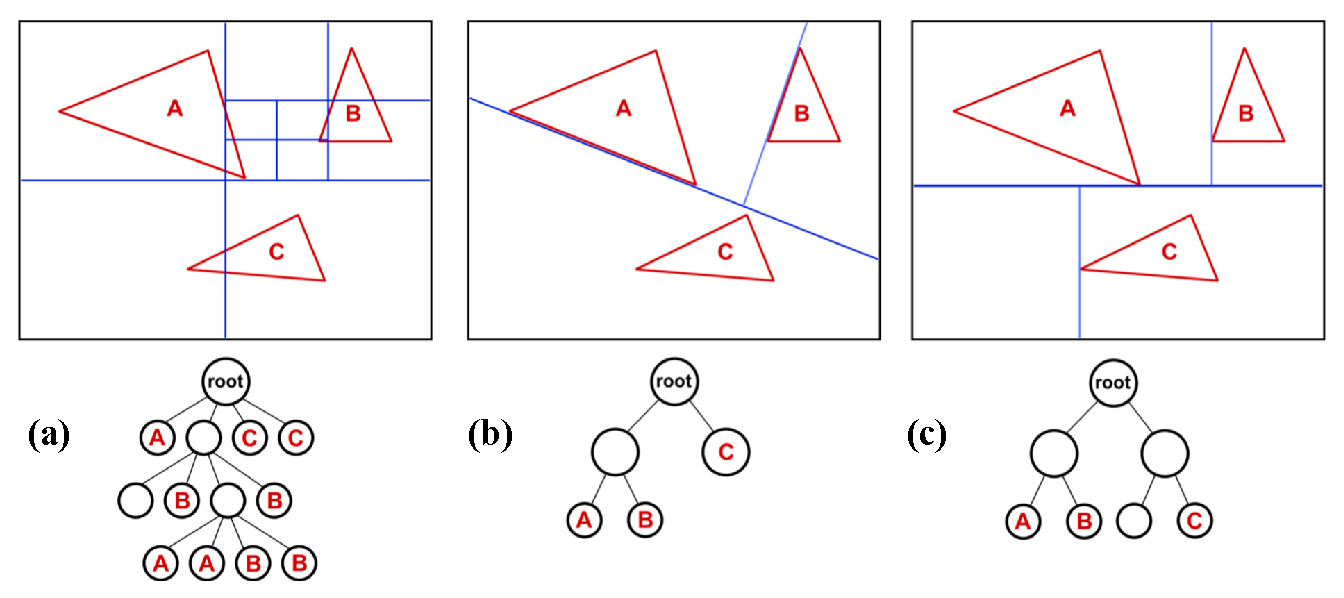
\includegraphics[width=1.\textwidth]{graphics/gi/path-17-1}
	\end{center}
	\caption{Spatial subdivisions: quadtree (2D equivalent of the octree), BSP, kD-tree (Image courtesy of J. Bikker).}
\end{figure}

An object subdivision subdivides the list of primitives, rather than space. Since primitives are split in such schemes, the space that primitives in different nodes of the hierarchy occupy may overlap. Examples of this class of acceleration structure are:

\begin{itemize}
	\item \textbf{BVH}, see figure \ref{f:object-subdivisions}a. Bounding Volume Hierarchies (BVH) recursively subdivides the list of objects, and stores, at each level of the tree, the bounds of the subtree. The bounds of two nodes at the same level in the tree may overlap. Nodes in the hierarchy cannot be empty. Most implementations implement the BVH as a binary tree. Some implementations however chose to split nodes in more than two sub-nodes. The QBVH and MBVH (we'll see in the following sections) use a maximum of four children per node.
	\item \textbf{BIH}, see figure \ref{f:object-subdivisions}b. The Bounding Interval Hierarchy is similar to the BVH, but rather than storing a full bounding box for each node, it stores intervals along one axis per node.
\end{itemize}

\begin{figure}\label{f:object-subdivisions}
	\begin{center}
		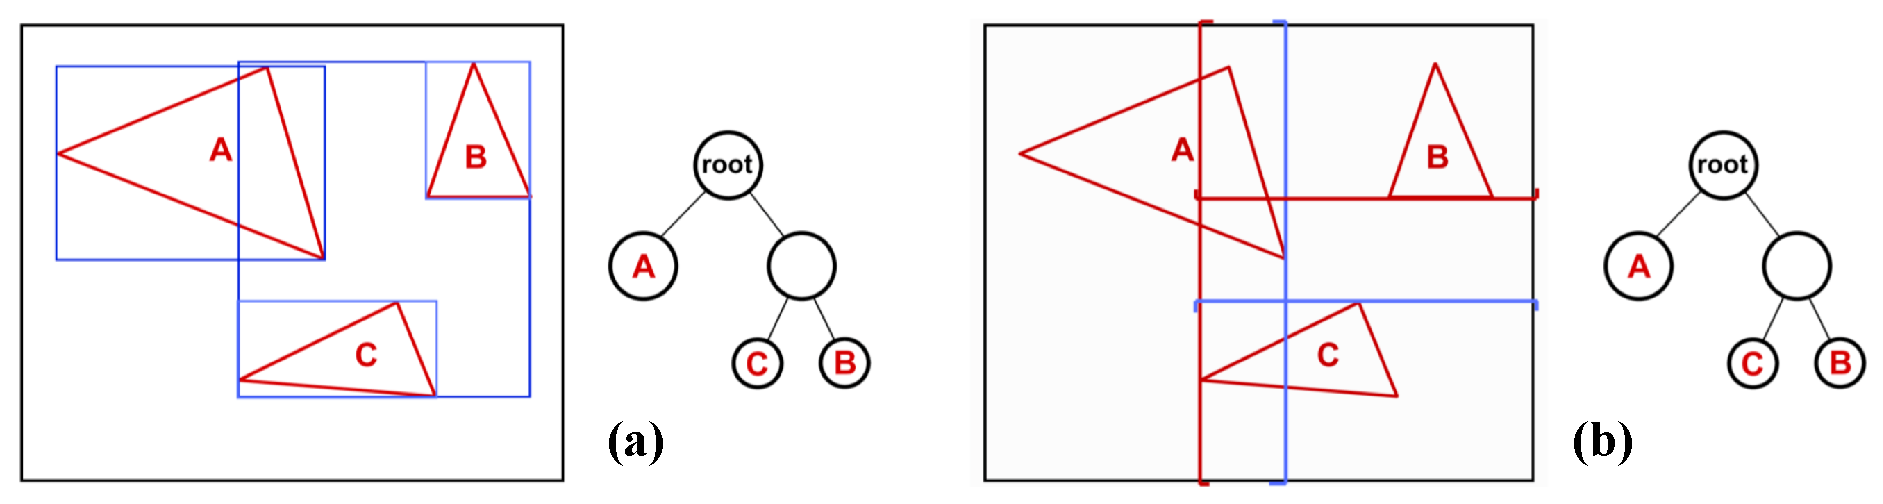
\includegraphics[width=1.\textwidth]{graphics/gi/path-17-2}
	\end{center}
	\caption{Object hierarchy: BVH and BIH (Image courtesy of J. Bikker).}
\end{figure}

While the kd-tree remains the best known acceleration structure for ray tracing of static scenes, BVH is more common. Most games use a scene graph to store object hierarchy and spatial relations between objects in the scene. This information can be exploited in two ways. First, the object bounding box planes provide good candidates for split planes near the root of a kD-tree or BVH. The cost of these initial splits can be dramatically reduced by considering only these planes. Secondly, for a BVH we can construct a BVH for each scene graph node. The scene BVH is then constructed using a top-level BVH over the scene graph node BVHs. That means we can dynamically change scenes and it's important to aim at real-time frame rates in a dynamical game world.



\subsection{Coherent Ray Tracing}\label{sec:coherent-ray-tracing}
Ray tracing has high computational cost, due to the need to traverse a scene with many rays, intersecting each with the geometric objects, shading the visible surface samples, and finally sending the resulting pixels to the screen. Before 2001, it even cannot challenge rasterization-based algorithms for interactive use.

Although ray tracing has the above disadvantage, it has more advantages which make Wald et al, believe that ray tracing is an interesting alternative even in the field of interactive 3D graphics. To improve the speed of ray tracing to the extent that it can compete with rasterization-based algorithms, they proposed a new algorithm \cite{a:InteractiveRenderingwithCoherentRayTracing} which makes better use of computational resources such as caches and SIMD instructions and better exploits image and object space coherence. As a result, they are able achieve interactive frame rates even on standard PCs.

They first discussed some general optimization techniques which has been applied to their ray tracing engine. They are:

\begin{itemize}
	\item \textbf{Code Complexity} A modern processor has several hardware features such as branch prediction, instruction reordering, speculative execution, etc, in order to avoid expensive pipeline stalls. These features need simple code that contains few conditional. So they optimize the ray traversal algorithm and make it shorter and simpler. They also choose to only support triangles as geometric primitives, so that the inner loop that performs intersection computations on list of objects does not have to branch to a different function for each type of primitive.
	\item \textbf{Caching} Their profiling reveals that a ray tracer is not bound by CPU speed, but is in fact bandwidth-bound by access to main memory. Especially shooting rays incoherently results in almost random memory accesses and bad cache performance.
		
		Since data transfer between memory and cache is always performed in entire cache lines of 32 bytes (now 64 bytes is more common), the \textit{effective} cost when accessing memory is not directly related to the number of bytes read, but the number of cache line transfers. 
		
		So they carefully align data to cache line: this minimizes the additional bandwidth requested to load two cache lines simply because some data happen to straddle a cache line boundary.
		
		They also keep data together if and only if it is used together: E.g. only data necessary for a triangle intersection test are stored in the geometry structures, while data that is only necessary for shading is stored separately.
	
	\item \textbf{Coherence through Packets of Rays} The most important aspect of accelerating ray tracing is to exploit coherence as far as possible. Their main approach is to exploit coherence of primary and shadow rays by traversing, intersecting, and shading \textit{packets of rays} in parallel. Using this approach they can reduce the compute time of the algorithm by using SIMD instructions on multiple rays in parallel, reduce memory bandwidth by requesting data only once per packet, and increase cache utilization at the same time.
\end{itemize}

Then they disscus the use of SIMD instructions to efficiently implement the main three components of a ray tracer: ray intersection computations, scene traversal, and shading. In 2001's paper they used a BSP acceleration structure, but they replaced it with a BVH structure to achieve a deformable scene needs in 2007 \cite{a:RayTracingDeformableScenesUsingDynamicBoundingVolumeHierarchies}. So we'll discuss the later.  

\begin{lstlisting}[language=C++,caption=A typical inner loop for BVH traversal,label=lst:single-ray-bvh]
while stack not empty
  if not leaf
    ray intersects far child ? push far child 
    ray intersects near child ? push near child
  else
    intersect primitives in leaf
  pop
\end{lstlisting}

\begin{lstlisting}[language=C++,caption=Basic ray packet traversal for a BVH,label=lst:packet-bvh]
while stack not empty
	if not leaf
		any ray intersects far child ? push far child 
		any ray intersects near child ? push near child
	else
		intersect primitives in leaf
	pop
\end{lstlisting}

The basic algorithm for single-ray BVH traversal is shown in algorithm \ref{lst:single-ray-bvh}. Ray packet traversal of a BVH requires a small modification to this algorithm: instead of visiting a node if a ray intersects it, the node is visited if any ray in the packet intersects it. This yields the conceptually simple algorithm \ref{lst:packet-bvh}: instead of traversing a node when a single ray intersects it, a node is visited when any ray intersects it.



\subsection{Sorted Deferred Shading and Hyperion} 
Although ray packet can improve performance, it focused on primary rays. Secondary rays are incoherent, which have more impact on performance than primary. We need more efficient method to deal with secondary rays.

In 2013, Christian Eisenacher et al, proposed \textit{sorted deferred shading}\cite{a:SortedDeferredShadingforProductionPathTracing} for production path tracing. In this paper, they introduced a novel two-stage ray sorting framework. First, \textbf{they sort large, potentially out-of-core ray batches} to ensure coherence; Second, \textbf{they sort ray hits for deferred shading with out-of-core textures}.

\begin{figure}\label{f:sorted-deferred-shading}
	\begin{center}
		\includegraphics[width=0.8\textwidth]{graphics/gi/path-10}
	\end{center}
	\caption{Left: It ensures coherent path tracing using two sorting stages; Right: An exploded view of ray sorting.}
\end{figure}

An overview of this path-tracing pipeline is given on the left of figure \ref{f:sorted-deferred-shading}. Starting with primary rays they perform \textbf{ray sorting}: They bin rays by direction and group them into large, sorted rays batches of fixed size, typically about 30-60M rays per batch. The OS streams inactive ray batches to a local SSD until the system is ready to sort and trace the next batch.

The next is performing \textbf{scene traversal}, one sorted ray batch at a time. They use a two-level quad-BVH with streaming packet traversal in the top level, and naive single-ray traversal in the bottom. The result of traversal is a list of hit points (one per ray).

Next, \textbf{hit point sorting} organizes ray hits by shading context. In Disney Animation Studio, they use a method, Ptex\cite[-10mm]{a:Ptex:Per-FaceTextureMappingforProductionRendering}, to store a separate texture per quad face of the subdivision control mesh, along with a novel per-face adjacency map, in a single texture file per surface. Thus, a full shading context consists of a mesh ID and a face ID, see figure \ref{f:ptex}. They group hit points by mesh ID, and then sort each group by face ID for coherent texturing and shading.

\begin{figure}\label{f:ptex}
	\sidecaption
	\includegraphics[width=0.65\textwidth]{graphics/gi/path-12}
	\caption{a) Portion of a control mesh showing intrinsic faceids and edgeids. b) Corresponding limit surface showing continuous isolines across faces.}
\end{figure}


\textbf{Shading} happens in parallel with each thread processing a different mesh. Because each mesh face is touched at most once when shading a ray batch, all shader inputs, including texture maps, are only accessed once. This amortizes per-file texture costs (opening the file over the network), and per-face texture costs (reading and decompressing a block of texels) perfectly for each batch. Further this access is coherent and sequential, so prefetching of subsequent per-face textures is trivial.

\begin{figure}\label{f:big-hero-6}
	\begin{center}
		\includegraphics[width=1.\textwidth]{graphics/gi/path-13}
	\end{center}
	\caption{Big Hero 6 was the first feature film which uses Hyperion, the new renderer of Walt Disney which use sorted deferred shading and other techniques (Image courtesy of Walt Disney Animation Studio).}
\end{figure}

This technique plus some other techniques, they called the new renderer \textit{Hyperion}, has been used in several films in Walt Disney Animation Studio, the first feature film was \textit{Big Hero 6}. In the film, the city San Fransokyo has 83,000 buildings built procedurally, plus a similar number of street props and trees. There are 216,000 street lights in the city instanced off six instanced based designs, see figure \ref{f:big-hero-6}.



\section{GPU Ray Tracing}
[Heitz14] Eric Heitz, Eugene D'Eon "Importance Sampling Microfacet-Based BSDFs using the Distribution of Visible Normals" https://hal.inria.fr/hal-00996995
[Hermanns15] Lukas Hermanns "Screen space cone tracing for glossy reflections" http://publica.fraunhofer.de/documents/N-336466.html
[Karis13] Brian Karis "Real Shading in Unreal Engine 4" http://blog.selfshadow.com/publications/s2013-shading-course/
[Karis14] Brian Karis "High-quality Temporal Supersampling" http://advances.realtimerendering.com/s2014/
[McGuire14] Morgan McGuire, Michael Mara "Efficient GPU Screen-Space Ray Tracing" http://jcgt.org/published/0003/04/04/
[Pearce15] William Pearce "Screen Space Glossy Reflections" http://roar11.com/2015/07/screen-space-glossy-reflections/
[Tokuyoshi15] Yusuke Tokuyoshi "Specular Lobe-Aware Filtering and Upsampling for Interactive Indirect Illumination" http://www.jp.square-enix.com/info/library/
[Uludag14] Yasin Uludag "Hi-Z Screen-Space Cone-Traced Reflections" GPU Pro 5
[Valient14] Michal Valient "Reflections And Volumetrics Of Killzone Shadow Fall" http://advances.realtimerendering.com/s2014/
